\documentclass[14pt]{article}

\usepackage[utf8x]{inputenc}
\usepackage[russian]{babel}
\usepackage{graphicx}
\graphicspath{{images/}}
\DeclareGraphicsExtensions{.pdf,.png,.jpg,.jpeg}

\usepackage{amsmath}
\usepackage{multirow}
\usepackage{pgfplots}

\usepackage{geometry} % Меняем поля страницы
\geometry{left=2cm}% левое поле
\geometry{right=1.5cm}% правое поле
\geometry{top=2cm}% верхнее поле
\geometry{bottom=2cm}% нижнее поле

\renewcommand{\theenumi}{\arabic{enumi}}% Меняем везде перечисления на цифра.цифра
\renewcommand{\labelenumi}{\arabic{enumi}}% Меняем везде перечисления на цифра.цифра
\renewcommand{\theenumii}{.\arabic{enumii}}% Меняем везде перечисления на цифра.цифра
\renewcommand{\labelenumii}{\arabic{enumi}.\arabic{enumii}.}% Меняем везде перечисления на цифра.цифра
\renewcommand{\theenumiii}{.\arabic{enumiii}}% Меняем везде перечисления на цифра.цифра
\renewcommand{\labelenumiii}{\arabic{enumi}.\arabic{enumii}.\arabic{enumiii}.}% Меняем везде перечисления на цифра.цифра

\begin{document}
\begin{titlepage}
	\begin{center}
		\fontsize{18pt}{20pt}\selectfont
		\textbf{Работа 1.4.4.}	
	
		\vspace{5cm}
		\fontsize{24pt}{25pt}\selectfont
		Исследование свободных колебаний связанных маятников
	\end{center}
	\begin{flushright}
		\fontsize{18pt}{20pt}\selectfont
		\vspace{14cm}
		\hspace{-3cm}
		\textit{Корнеев Е.С.}
	\end{flushright}		
\end{titlepage}

\begin{center}
	\fontsize{16pt}{18pt}\selectfont	
	Исследование свободных колебаний связанных маятников
\end{center}

\fontsize{14pt}{16pt}\selectfont
\vspace{1cm}
\textbf{Цель работы:} изучение колебательной системы с двумя степенями свободы.

\vspace{0.5cm}
\textbf{В работе используются:} устновка с двумя одинаковыми математическими маятниками, бифилярно подвещенными на натянутую горизонтально струну, секундомер, измерительная линейка.

\vspace{1cm}
\textbf{Свободные колебания связанных маятников. Теоретические основы.} Рассмотрим простейшую модель с двумя степенями свободы --- два одинаковых маятника, связанных пружиной и совершающих колебания в плоскости рисунка. Маятники представляют собой невесомые спицы с насаженными на них маленькими тяжелыми шариками.

Обозначения указаны на рисунке. Если углы отклонения маятника от положения равновесия достаточно малы 
($\sin\varphi \approx \varphi,~\cos\varphi \approx 1 - \varphi/2$), то со стороны пружины на первый маятник действует момент силы, равный

$$M_{21} = ka^2(\varphi_2 - \varphi_1)$$

\noindent Аналогично второй маятник будет испытывать вращающий момент противоположного знака:

$$M_{12} = -ka^2(\varphi_2 - \varphi_1)$$

\noindent Эти моменты описывают связь между маятниками.

Уравнения движения матяником имеют вид

\begin{equation}\label{fluct_eq_1}
ml^2\frac{d^2\varphi_1}{dt^2} = -mgl\varphi_1 + ka^2(\varphi_2 - \varphi_1)
\end{equation}	
\begin{equation}\label{fluct_eq_2}
ml^2\frac{d^2\varphi_2}{dt^2} = -mgl\varphi_2 - ka^2(\varphi_2 - \varphi_1)
\end{equation}

\noindent Сложив эти два уравнения, находим

\begin{equation}\label{fluct_sum}
ml^2\frac{d^2}{dt^2}(\varphi_1 + \varphi_2) = -mgl(\varphi_1 + \varphi_2)
\end{equation}

Вычитание (\ref{fluct_eq_2}) - (\ref{fluct_eq_1}) дает

\begin{equation}\label{fluct_div}
ml^2\frac{d^2}{dt^2}(\varphi_1 - \varphi_2) = -(mgl + 2ka^2)(\varphi_1 - \varphi_2)
\end{equation}


\begin{figure}[h!]
	\center{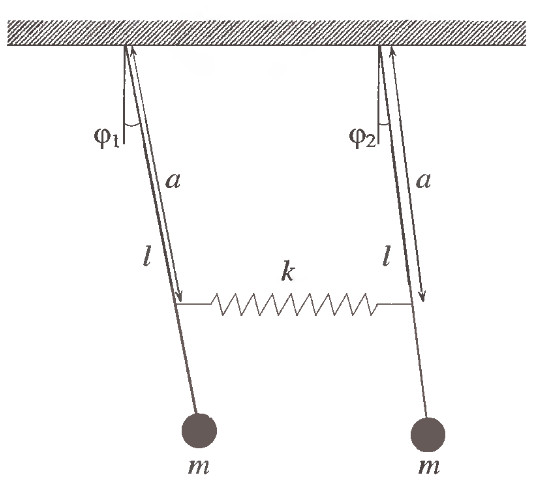
\includegraphics[width = 9cm]{pendulums}}
	\caption{Связанные маятники}
	\label{fig:image}
\end{figure} 


Решения уравнений (\ref{fluct_eq_1}) и (\ref{fluct_eq_2}) имеют вид:

\begin{equation}\label{fluct_eq_solve_1}
\varphi_1 + \varphi_2 = A\cos(\omega^+t + \alpha)
\end{equation}
\begin{equation}\label{fluct_eq_solve_2}
\varphi_1 - \varphi_2 = B\cos(\omega^-t + \beta)
\end{equation}

$$\omega^+ = \sqrt{\frac{g}{l}}, ~ \omega^- = \sqrt{\frac{g}{l} + \frac{2ka^2}{ml^2}}$$

\noindent где $A, B, \alpha, \beta$ - произвольные константы. Сладывая и вычитая (\ref{fluct_eq_solve_1}) и (\ref{fluct_eq_solve_2}), находим

\begin{equation}\label{ph_1}
\varphi_1 = \frac{1}{2}A\cos(\omega^+t + \alpha) + \frac{1}{2}B\cos(\omega^-t + \beta)
\end{equation}
\begin{equation}\label{ph_2}
\varphi_2 = \frac{1}{2}A\cos(\omega^+t + \alpha) - \frac{1}{2}B\cos(\omega^-t + \beta)
\end{equation}

\noindent Для угловых скоростей при этом имеем

\begin{equation}\label{dot_phi_1}
\dot \varphi_1 = -\frac{1}{2}A\sin(\omega^+t + \alpha) - \frac{1}{2}B\sin(\omega^-t + \beta)
\end{equation}
\begin{equation}\label{dot_phi_2}
\dot \varphi_2 = -\frac{1}{2}A\sin(\omega^+t + \alpha) + \frac{1}{2}B\sin(\omega^-t + \beta)
\end{equation}

Проанализируем полученные решения. Пустья маятники имеют вначале (при $t = 0$) одинаковые отклонения и нулевые начальные скорости:

$$\varphi_1(0) = \varphi_2(0) = \varphi_0, ~~\dot \varphi_1(0) = \dot \varphi_2(0) = 0$$

\noindent Тогда из (\ref{ph_1})---(\ref{dot_phi_2}) находим

$$\sin\alpha = 0, ~~A = 2\varphi_0, ~~B = 0$$

\noindent то есть

\begin{equation}\label{ph_1, ph_2, 1}
\varphi_1 = \varphi_0\cos\omega^+t, ~~\varphi_2 = \varphi_0\cos\omega^+t
\end{equation}

\noindent Этоозначает, что маятники буду колебаться с одинкаковой амплитудой и в одинаковой фазе.

Если при $t = 0$

$$\varphi_1(0) = -\varphi_2(0) = \varphi_0, ~~\dot \varphi_1(0) = \dot \varphi_2(0) = 0$$

\noindent то из (\ref{ph_1})---(\ref{dot_phi_2}) следует

$$\sin\beta = 0, ~~A = 0, ~~B = 2\varphi_0$$

\noindent то есть

\begin{equation}\label{ph_1, ph_2, 2}
\varphi_1 = \varphi_0\cos\omega^-t, ~~\varphi_2 = -\varphi_0\cos\omega^-t = \varphi_0\cos(\omega^-t + \pi)
\end{equation}

Соотношения показывают, что маятники колеблются с одинаковой амплитудой, синхронно, но не синфазно: колебания матяников находятся в противофазе. Два вида движения (\ref{ph_1, ph_2, 1}) и (\ref{ph_1, ph_2, 2}) называются нормальными модами колебаний системы связанных осцилляторов. Нормальная мода колебаний - это коллективное колебание, при котором амплитуда колебаний каждой частицы остается постоянной. В современной физике понятие моды играет очень важную роль.

Рассмотрим теперь случай, когда в начальный момент времени отклонен лишь один маятник, т. е.

$$\varphi_1(0) = \varphi_0, ~~\varphi_2(0) = 0, ~~\dot \varphi_1(0) = \dot \varphi_2(0) = 0$$



Можно показать, что в этом случае 

\begin{equation}\label{protivofaza_1}
\varphi_1 = \frac{\varphi_0}{2}(\cos\omega^+t + \cos\omega^-t)
\end{equation}
\begin{equation}\label{protivofaza_2}
\varphi_1 = \frac{\varphi_0}{2}(\cos\omega^+t - \cos\omega^-t)
\end{equation}

\noindent Уравнения (\ref{protivofaza_1}), (\ref{protivofaza_2}) можно представить в виде

\begin{equation}\label{ph_1 solve}
\varphi_1 = \varphi_0\cos\frac{\omega^+ - \omega^-}{2}t \cdot \cos\frac{\omega^+ + \omega^-}{2}t
\end{equation}
\begin{equation}\label{ph_2 solve}
\varphi_2 = \varphi_0\sin\frac{\omega^+ - \omega^-}{2}t \cdot \sin\frac{\omega^+ + \omega^-}{2}t
\end{equation}

Проанализируем формулы (\ref{ph_1 solve}) и (\ref{ph_2 solve}). Заметим, что частота колебаний четной моды $\omega^+ = \sqrt{g/l}$ равна 
$\omega_0$, где $\omega_0$ - собственная частота одиночного маятника (так называемая парциальная частота). С другой стороны, частота колебаний нечетной моды равна $\omega^- = \omega_0\sqrt{1 + 2\varepsilon	}$, где параметр $\varepsilon = ka^2/mgl$ характеризует связь маятников. В случае слабой связи, когда $\varepsilon \ll 1$, можно считать, что $\omega^- \approx \omega_0(1 + \varepsilon)$, т. е.

$$\omega^- - \omega^+ \approx \omega_0\varepsilon, ~~\omega^- + \omega^+ \approx 2\omega_0$$

Уравнения (\ref{ph_1 solve}) и (\ref{ph_2 solve}) при этом можно приближенно представить в виде

\begin{equation}
\varphi_1 = \varphi_0\cos\frac{\omega_0\varepsilon}{2}t \cos\omega_0t
\end{equation}
\begin{equation}
\varphi_2 = \varphi_0\sin\frac{\omega_0\varepsilon}{2}t \sin\omega_0t = 
\varphi_0\sin\frac{\omega_0\varepsilon}{2}t \cos(\omega_0t - \frac{\pi}{2})
\end{equation}

\noindent Таким образом, мы имеем дело с гармоническими колебаниями частоты $\omega_0$, амплитуда которых изменяется со временем периодически с сильно меньшей частотой $\omega_0\varepsilon/2$. Это так называемые амплитудно-модулированные колебания, или биения. Относительная фаза колебаний равна $\pi/2$. Модулированная амплитуда колебаний первого маятника есть величина

$$A_1(t) = \varphi_0\cos\frac{\omega_0\varepsilon}{2}t$$

\noindent Аналогично амплитуда колебаний второго маятника равна

$$A_2(t) = \varphi_0\sin\frac{\omega_0\varepsilon}{2}t = \varphi_0\cos(\frac{\omega_0\varepsilon}{2}t - \frac{\pi}{2})$$

\noindent В начальный момент времени $t = 0$ имеем

$$A_1 = \varphi_0, ~~~A_2 = 0$$

\noindent В момент времени $t = \pi/\omega_0\varepsilon$

$$A_1 = 0, ~~~A_2 = \varphi_0$$

\noindent В момент времени $t = 2\pi/\omega_0\varepsilon$

$$A_1 = -\varphi_0, ~~~A_2 = 0$$

\noindent Отметим, что амплитуда гармонического колебания, по определнию, величина положительная. Отрицательный знак означает, что относительная амплитуда изменилась на $\pi$. В момент времени $t = 3\pi/\omega_0\varepsilon$

$$A_1 = 0, ~~~A_2 = -\varphi_0$$

\noindent В момент времени $t = 4\pi/\omega_0\varepsilon$ имеем

$$A_1 = \varphi_0, ~~~A_2 = 0$$

Таким образом, происходит передача колебаний от одного маятника к другому. Маятники обладают энергией. При $t = 0$ вся энергия сосредоточена в одном маятнике. В результате связи через пружину энергия постепенно передается от первого маятника ко второму до тех пор, пока в нем не накопится вся энергия. Время $\tau$, необходимое для перехода энергии от одного маятника к другому и обратно, можно оценить из уравнения

$$\frac{\omega_0\varepsilon}{2}\tau = \pi$$

\noindent т. е.

\begin{equation}\label{tau}
\tau = \frac{2\pi}{\omega_0\varepsilon}
\end{equation}

Частота, с которой маятники обмениваются энергией, равна

$$\frac{2\pi}{\tau} = \omega_0\varepsilon = \omega^- - \omega^+$$

Отметим, что колебания в системе с большим числом связанных осцилляторов можно трактовать как распространение в системе определенного типа волн.


\setcounter{equation}{0}
\newpage

%
% Here is new part of the book taken from 1.4.4.
%

\textbf{Лабораторная работа.}

Измерения проводятся на установке, изображенной на на рис. 1.

Один конец струны прикреплен к вертикальной стойке установки, а другой конец переброшен через неподвижный блок и натянут при помощи груза массы 
$M$. Точки струны $A$ и $B$ неподвижны. В точках $C$ и $D$, которые делят расстояние между $A$ и $B$ на три равные части (каждая длиной $a$), подвешены одинаковые математические маятники массой $m$ и длиной $l$. Каждый маятник подвешен на двух нитях в плоскости струны (бифилярно), чтобы колебания мятников проходили в плоскостях, перпендикулярных струне. Сила натяжения струны намного больше веса матяников ($M \gg m$). Вертикальная составляющая смещения струны никак не сказывается на движении маятников при малых отклонениях. Горизонтальная составляющая смещения струны, хоть она и мала по сравнению со смещениями маятников, осуществляет слабую связь между маятниками.

На рис. 2. показаны смещения точек $C$ и $D$ струны и отклонения маятников в вертикальной (рис. 2а) и горизонтальной (рис. 2б) плоскостях. 

При небольших отклонениях маятников для силы натяжения подвеса маятника $T$ имеем (рис. 2а)

\begin{equation}
mg \approx T
\end{equation}

Для движения матяников в горизонтальном направлении (рис. 2)

\begin{equation}
m\ddot x_1 = -T\sin\varphi_1 \approx -T\frac{x_1 - x_3}{l} \approx -mg\frac{x_1 - x_3}{l}
\end{equation}
\begin{equation}
m\ddot x_2 = -T\sin\varphi_2 \approx -T\frac{x_2 - x_4}{l} \approx -mg\frac{x_2 - x_4}{l}
\end{equation}

\begin{figure}[h!]
	\center{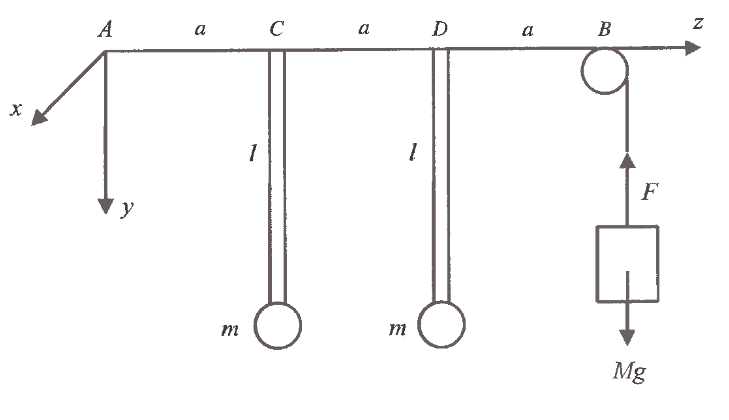
\includegraphics[width = 12cm]{scheme1}}
	\caption{Общий вид установки}
	\label{fig:image}
\end{figure}

\begin{figure}[h!]
	\center{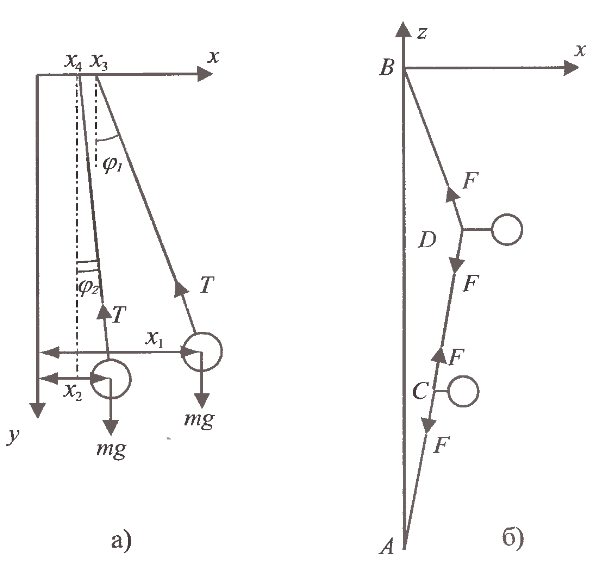
\includegraphics[width = 12cm]{scheme2}}
	\caption{
		Отклонения маятников и струны:
		а) вид вдоль струны
		б) вид вид сверху	
	}
	\label{fig:image}
\end{figure}

Связь между натяжением струны и натяжением подвеса получаем из рис. 2:

\begin{equation}
T\frac{x_1 - x_3}{l} = F\frac{x_3}{a} + F\frac{x_3 - x_4}{a}
\end{equation}
\begin{equation}
T\frac{x_2 - x_4}{l} = F\frac{x_4}{a} + F\frac{x_4 - x_3}{a}
\end{equation}

Введем безразмерный параметр

$$
\sigma = \frac{T}{F} \frac{a}{l} = \frac{m}{M}\frac{a}{l}
$$

\noindent который в нашем случае много меньше единицы (связь слабая). Тогда из (4) и (5) получаем

\begin{equation}
\sigma x_1 = (2 + \sigma)x_3 - x_4,~~\sigma x_2 = (2 + \sigma)x_4 - x_3
\end{equation}

\noindent пренебрегая $\sigma$ по сравнению с 2, получаем

\begin{equation}
x_3 = \sigma\frac{2x_1 + x_2}{3},~~ x_4 = \sigma\frac{x_1 + 2x_2}{3}
\end{equation}

Уравнения движения маятников примут вид

\begin{equation}\label{x_1 fluct equation}
\ddot x_1 + \frac{g}{l}(1 - \sigma)x_1 = \sigma\frac{g}{3l}(x_2 - x_1)
\end{equation}
\begin{equation}\label{x_2 fluct equation}
\ddot x_2 + \frac{g}{l}(1 - \sigma)x_2 = \sigma\frac{g}{3l}(x_1 - x_2)
\end{equation}

Заметим, что система уравнений (\ref{fluct_eq_1}), (\ref{fluct_eq_2}) из предыдущего раздела может быть записана в виде

$$
\ddot \varphi_1 + \frac{h}{l}\varphi_1 = \frac{g}{l}\varepsilon(\varphi_2 - \varphi_1)
$$
$$
\ddot \varphi_2 + \frac{h}{l}\varphi_2 = \frac{g}{l}\varepsilon(\varphi_1 - \varphi_2)
$$

\noindent или

\begin{equation}\label{phi_1 fluct equation}
\ddot \varphi_1 + \omega_0^2\varphi_1 = \omega_0^2\varepsilon(\varphi_2 - \varphi_1)
\end{equation}
\begin{equation}\label{phi_2 fluct equation}
\ddot \varphi_2 + \omega_0^2\varphi_2 = \omega_0^2\varepsilon(\varphi_1 - \varphi_2)
\end{equation}

\noindent Уравнения (\ref{phi_1 fluct equation}), (\ref{phi_2 fluct equation}) с точностью до обозначений совпадают с уравнениями 
(\ref{x_1 fluct equation}), (\ref{x_2 fluct equation}). Введем обозначения 

$$
\frac{g}{l}(1 - \sigma) = \omega_0^2, ~~\sigma\frac{g}{3l} = \omega_0^2\varepsilon
$$

\noindent Откуда

$$
\frac{\sigma}{1 - \sigma} = 3\varepsilon
$$

\noindent или

$$
\sigma(1 + \sigma) \approx 3\varepsilon
$$

\noindent т. е.

$$
\sigma \approx 3\varepsilon ~~(\text{для слабой связи})
$$

\noindent Система уранений (\ref{x_1 fluct equation}), (\ref{x_2 fluct equation}) принимает вид

\begin{equation}
\ddot x_1 + \omega_0^2x_1 = \omega_0^2\varepsilon(x_2 - x_1)
\end{equation}

\begin{equation}
\ddot x_2 + \omega_0^2x_2 = -\omega_0^2\varepsilon(x_2 - x_1)
\end{equation}

Из теоретического введения (\ref{tau}):

$$
\tau = \frac{2\pi}{\omega_0\varepsilon}
$$

\noindent Можно видеть, что параметр связи 

$$
\varepsilon = \frac{1}{3}\left( 1 - \frac{\omega_0^2l}{g} \right)
$$

\noindent В силу последнего:

\begin{equation}\label{last}
\tau = \frac{6\pi}{\omega_0(1 - \omega_0^2l/g)} \approx 6\pi\frac{Ml}{ma}\sqrt{\frac{l}{g}}
\end{equation}

\noindent Формулу (\ref{last}) можно проверить экспериментально.

\newpage
\textbf{Наши действия.}
\vspace{1cm}

\begin{flushleft}
\begin{enumerate}
\item Измерим длину маятников, расстояние между неподвижными точками струны и точками повеса маятников. Запишем массу маятников и массу груза, натягивающего струну.
\item Измерим приоды мод. Для измерения периода $T_1$ синфазных колебаний маятников отклоним их на одинаковые углы (примерно $30^{\circ}$) в одну сторону и одновременно отпустим. Повторим измерения несколько раз и усредним результаты, аналогично измерим период колебаний $T_2$ в противофазе, отклоняя маятники в разные стороны.
\item Измерим период парциальных колебаний, отцепив один из маятников.
\item Измерим период биений, проверим справедливость соотношения

$$
	\frac{1}{\tau} = \frac{1}{T_2} - \frac{1}{T_1}
$$

\item Повторим предыдущие измерения при других натяжениях струны.
\item Построим график зависимости периода биений от натяжения струны.
\item Проведем сравнение полученных результатов с теоретическими рассчетами по формуле (\ref{last}).
\end{enumerate}
\end{flushleft}

\newpage
\textbf{Измерения}
\vspace{1cm}

Определим параметры установки:

\begin{center}
\begin{tabular}{|c|c|c|c|c|c|c|}
\hline
Расстояние между точками подвеса маятников $a$		&	25	см	\\
\hline
Длина маятников $l$									&	45	см	\\
\hline
Масса маятников $m$									&	225	см	\\
\hline
\end{tabular}
\end{center}

Измерим периоды нескольких колебаний $T_1$ и $T_2$, $\tau$, а также вычислим, чему должно равняться значение $\tau_0$ согласно формуле проверяемой зависимости для различных масс $M$, добавляемых к грузу, натягивающему трос.

\begin{center}
\begin{tabular}{|c|c|c|c|c|c|c|c|c|c|c|}
\hline
\multicolumn{3}{|c|}{$M = 95$ г}	\\
\hline
$10\cdot T_1$, c	&	$10\cdot T_2$, c			&	$\tau$, c				\\
\hline
14.02				&	13.56						&	39						\\
\hline
14.01				&	13.52						&	38						\\
\hline
14.01				&	13.48						&	40						\\
\hline
14.00				&	13.52						&	39						\\
\hline
14.02				&	13.51						&							\\
\hline
14.00				&	13.53						&							\\
\hline
$T_1 = (1.401 \pm 0.001)$c		&	$T_2 = (1.352 \pm 0.002)$c		&	$\tau = (39 \pm 1)$c	\\
\hline
\multicolumn{3}{|c|}{$\tau_0 = (38 \pm 2)$c}								\\
\hline
\end{tabular}
\end{center}

\begin{center}
\begin{tabular}{|c|c|c|c|c|c|c|c|c|c|c|}
\hline
\multicolumn{3}{|c|}{$M = 503$ г}	\\
\hline
$10\cdot T_1$, c	&	$10\cdot T_2$, c			&	$\tau$, c				\\
\hline
13.88				&	13.49						&	50						\\
\hline
13.89				&	13.48						&	50						\\
\hline
13.85				&	13.48						&	51						\\
\hline
13.88				&	13.52						&	49						\\
\hline
13.89				&	13.51						&							\\
\hline
$T_1 = (1.388 \pm 0.001)$c		&	$T_2 = (1.350 \pm 0.001)$c		&	$\tau = (50 \pm 1)$c	\\
\hline
\multicolumn{3}{|c|}{$\tau_0 = (49 \pm 3)$c}									\\
\hline
\end{tabular}
\end{center}

\begin{center}
\begin{tabular}{|c|c|c|c|c|c|c|c|c|c|c|}
\hline
\multicolumn{3}{|c|}{$M = 984$ г}	\\
\hline
$10\cdot T_1$, c	&	$10\cdot T_2$, c			&	$\tau$, c				\\
\hline
13.77				&	13.42						&	62						\\
\hline
13.79				&	13.40						&	60						\\
\hline
13.78				&	13.44						&	63						\\
\hline
13.73				&	13.43						&	62						\\
\hline
13.70				&	13.40						&							\\
\hline
13.72				&	13.42						&							\\
\hline
$T_1 = (1.375 \pm 0.003)$c		&	$T_2 = (1.342 \pm 0.001)$c		&	$\tau = (62 \pm 1)$c	\\
\hline
\multicolumn{3}{|c|}{$\tau_0 = (56 \pm 6)$c}									\\
\hline
\end{tabular}
\end{center}

\begin{center}
\begin{tabular}{|c|c|c|c|c|c|c|c|c|c|c|}
\hline
\multicolumn{3}{|c|}{$M = 1996$ г}	\\
\hline
$20\cdot T_1$, c	&	$10\cdot T_2$, c			&	$\tau$, c				\\
\hline
27.30				&	13.30						&	80						\\
\hline
27.32				&	13.40						&	81						\\
\hline
27.20				&	13.45						&	80						\\
\hline
27.25				&	13.38						&	79						\\
\hline
27.27				&	13.40						&							\\
\hline
$T_1 = (1.364 \pm 0.001)$c		&	$T_2 = (1.339 \pm 0.004)$c		&	$\tau = (80 \pm 2)$c	\\
\hline
\multicolumn{3}{|c|}{$\tau_0 = (73 \pm 15)$c}									\\
\hline
\end{tabular}
\end{center}

\begin{center}
\begin{tabular}{|c|c|c|c|c|c|c|c|c|c|c|}
\hline
\multicolumn{3}{|c|}{$M = 3267$ г}	\\
\hline
$10\cdot T_1$, c	&	$10\cdot T_2$, c			&	$\tau$, c				\\
\hline
13.40				&	13.33						&	102						\\
\hline
13.55				&	13.36						&	99						\\
\hline
13.55				&	13.37						&	100						\\
\hline
13.42				&	13.38						&	100						\\
\hline
13.52				&	13.30						&							\\
\hline
13.45				&	13.33						&							\\
\hline
$T_1 = (1.348 \pm 0.006)$c		&	$T_2 = (1.335 \pm 0.003)$c		&	$\tau = (100 \pm 2)$c	\\
\hline
\multicolumn{3}{|c|}{$\tau_0 = (138 \pm 95)$c}									\\
\hline
\end{tabular}
\end{center}




\begin{center}
\begin{tikzpicture}
\begin{axis}[
	height = 9cm,
	width  = 14cm,
	every axis y label/.style={at = {(ticklabel cs: 0.5)}, rotate = 90, anchor = near ticklabel},
	xlabel = {$M, \text{г}$},
	ylabel = {$\tau, \text{с}$}
]
\addplot+[only marks,
	error bars/.cd, 
	y dir = both, y explicit,
	x dir = both, x explicit,
	]
coordinates{
	(  95, 39 ) +- (0, 1)
	( 503, 50 ) +- (0, 1)
	( 984, 62 ) +- (0, 2)
	(1996, 80 ) +- (0, 2)
	(3276, 100) +- (0, 2)
};
\addplot+[only marks,
	error bars/.cd, 
	y dir = both, y explicit,
	x dir = both, x explicit,
	]
coordinates{
	(  95, 38 ) +- (0, 2)
	( 503, 49 ) +- (0, 3)
	( 984, 56 ) +- (0, 6)
	(1996, 73 ) +- (0, 15)
	%(3276, 138) +- (0, 95)
};

% OLS

\addplot [mark = none]
coordinates{
	(95, 42.1665)
	(3276, 102.09)
};
\addplot [mark = none]
coordinates{
	(95, 32.65)
	(3276, 127.771)
};
\end{axis}
\end{tikzpicture}
\end{center}

\vspace{1cm}
По формуле (\ref{last})
$$
	\frac{\tau}{M} = 6\pi\frac{l}{ma}\sqrt{\frac{l}{g}} \approx 30~\text{с/кг}
$$

Определим угловой коэффициент графиков $k_1$ и $k_2$:
$$
	k_1 = 20 \pm 5~\text{с/кг}
$$
$$
	k_2 = 33 \pm 8~\text{с/кг}
$$

\vspace{1cm}
Видно, что угловые коэффициентыпрямых, полученных экспериментально и теоретически, близки к значению, вычисленному по формуле, спарведливость которой мы устанавливали. Учитывая погрешности, величина которых в данной лабораторной работе довольно велика, можно считать, что полученное значение вполне подтверждает полученную теоретическую зависимость, в связи с чем можно считать, что она с достаточной точностью описывает явления, наблюдаемые на практике.

\newpage
Список использованной литературы:
	
\vspace{0.5cm}
1. "Лабораторный практикум по общей физике: Учебное пособие. В трех томах. Т1. Механика"/А.Д.Гладун, Д.А.Александров,
Ф.Ф.Игошин и др.; Под редакцией А.Д.Гладуна. --- МФТИ, 2004.

2. "Набор и верстка в системе \LaTeX "/С.М.Львовский. --- 2003.

\end{document}